\documentclass[tikz,border=2pt]{standalone}
\usepackage[T1]{fontenc}
\usepackage{lmodern,amsmath,pgfplots}
\usetikzlibrary{arrows.meta,positioning}
\pgfplotsset{compat=1.18}
\begin{document}
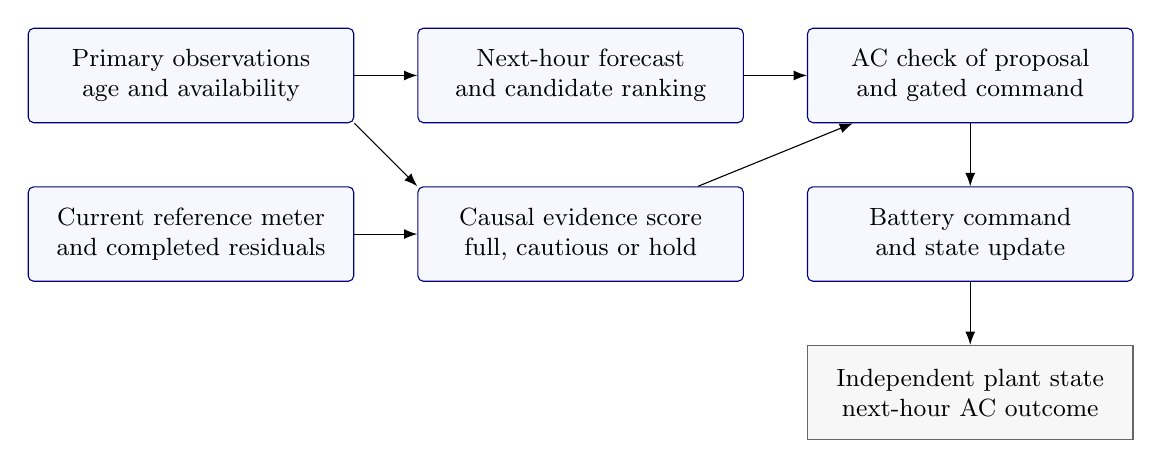
\begin{tikzpicture}[node distance=8mm and 8mm,>=Latex,
 box/.style={draw=blue!50!black,rounded corners=2pt,fill=blue!3,align=center,font=\small,minimum height=12mm,text width=39mm},
 eval/.style={draw=black!60,fill=black!3,align=center,font=\small,minimum height=12mm,text width=39mm}]
\node[box] (obs) {Primary observations\\age and availability};
\node[box,right=of obs] (pred) {Next-hour forecast\\and candidate ranking};
\node[box,right=of pred] (check) {AC check of proposal\\and gated command};
\node[box,below=of obs] (ref) {Current reference meter\\and completed residuals};
\node[box,right=of ref] (score) {Causal evidence score\\full, cautious or hold};
\node[box,right=of score] (command) {Battery command\\and state update};
\node[eval,below=of command] (plant) {Independent plant state\\next-hour AC outcome};
\draw[->] (obs)--(pred);\draw[->] (pred)--(check);
\draw[->] (obs.south east)--(score.north west);
\draw[->] (ref)--(score);\draw[->] (score)--(check);
\draw[->] (check)--(command);\draw[->] (command)--(plant);
\end{tikzpicture}
\end{document}
